\chapter{总图：从光子到点云的误差预算}
\label{ch:11}

前面各章分别讨论了几何成像、相机模型、标定、波动光学、偏振、辐射度量、结构光、三角测量、$\MTF$ 与其他深度传感。本章把它们串成一条链：一个光子从光源出发，经过场景、镜头、传感器，变成相位或匹配，再经三角测量变成点云中的一个点。每一环都向最终误差贡献一份，预算的任务就是逐项列出、区分性质、找出最大项。

\section{效果}
\label{sec:ch11-effect}

读完本章，你应能：
\begin{enumerate}
  \item 画出从光子到点云的误差链，并说出每一环对应的章节与主要误差项；
  \item 区分随机项与系统项，说明哪些可以靠平均降低、哪些必须靠建模或改设计；
  \item 用一张误差预算表给出单点深度误差的量级，并按平方和或线性叠加合成；
  \item 根据重建中出现的症状反查最可能的环节与章节；
  \item 对一个完整的结构光系统设计做综合取舍。
\end{enumerate}

\section{原理}
\label{sec:ch11-principle}

\subsection{误差链}

图~\ref{fig:ch11-map} 给出整条链。按顺序：
\begin{enumerate}
  \item \textbf{光源与投影}（第~\ref{ch:05}~章、第~\ref{ch:07}~章）：光谱、相干性（散斑）、伽马、DMD 比特面与帧同步、亮度漂移。
  \item \textbf{场景}（第~\ref{ch:05}~章、第~\ref{ch:07}~章）：镜面高反、次表面散射、互反射、偏振状态变化、运动。
  \item \textbf{镜头}（第~\ref{ch:01}~章、第~\ref{ch:02}~章、第~\ref{ch:03}~章、第~\ref{ch:04}~章、第~\ref{ch:09}~章）：$\PSF$/$\MTF$、景深与离焦、畸变、色差、衍射极限。
  \item \textbf{传感器}（第~\ref{ch:06}~章）：光子散粒噪声、读出噪声、暗电流、饱和、非线性响应、曝光控制。
  \item \textbf{相位或匹配}（第~\ref{ch:04}~章、第~\ref{ch:07}~章）：$\sigma_\varphi$、展开错误、伽马谐波、混合像素。
  \item \textbf{三角测量}（第~\ref{ch:02}~章、第~\ref{ch:03}~章、第~\ref{ch:08}~章）：$Z^2/(Bf_x)$ 放大、内参与外参误差、畸变残差、温漂。
  \item \textbf{点云}：多帧融合、拼接累积、滤波与网格化。
\end{enumerate}

\begin{figure}[htbp]
  \centering
  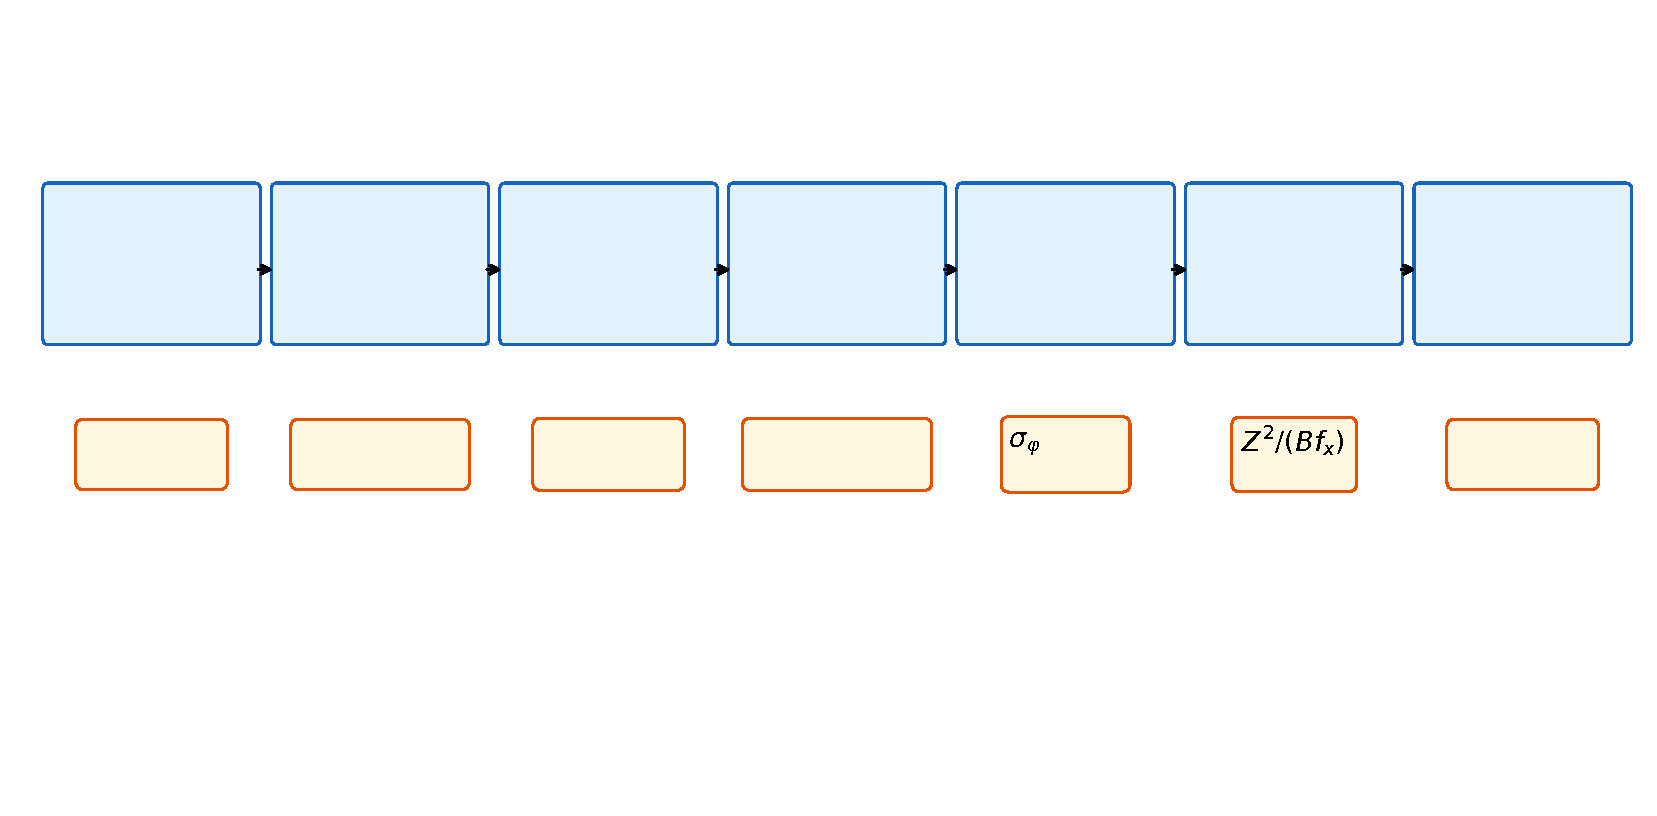
\includegraphics[width=\textwidth]{fig-error-budget-map.pdf}
  \caption{从光子到点云的误差链与各环节主要误差项、对应章节（概念草图，非精确工程图）。}
  \label{fig:ch11-map}
\end{figure}

\subsection{随机项与系统项}

\textbf{随机项}在重复测量间独立变化，均值为零：光子噪声、读出噪声、散斑（换照明位置后变化时）、量化噪声。它们按 $1/\sqrt{n}$ 随平均帧数 $n$ 降低，也随 $\SNR$ 提高而降低。

\textbf{系统项}在重复测量间保持不变，或随某个条件（深度、视场位置、材料、温度）确定性地变化：标定误差、残余畸变、伽马谐波、次表面散射偏置、色差、混合像素、展开错误。平均对它们无效；只能通过更好的模型（标定、补偿）、改变测量条件（换波长、换频率、交叉偏振），或改变设计来降低。

两点值得强调：
\begin{itemize}
  \item 同一现象可兼具两种成分。例如散斑：固定照明下对静止物体是系统项（每次都一样），移动照明或物体后变为随机项。
  \item 系统项常有\emph{空间结构}：碗形、周期波纹、台阶、尺度偏差。这一结构正是诊断的线索。
\end{itemize}

\subsection{误差合成}

相互独立的随机项按平方和合成：
\begin{equation}
  \sigma_{Z,\mathrm{rand}}=\sqrt{\sum_i\sigma_{Z,i}^{2}}.
  \label{eq:ch11-rss}
\end{equation}
系统项若方向与大小已知，应直接补偿；若只知道上界，保守做法是线性相加，较乐观的做法是视为未知但独立后按平方和合成。最终报告建议分开给出随机部分与系统部分，而不是只给一个数。

把各环节换算到深度，常用的「换算因子」是：
\begin{itemize}
  \item 灰度噪声 $\to$ 相位：$\sigma_\varphi\approx\sqrt{2/N}\,\sigma_I/M$（第~\ref{ch:07}~章）；
  \item 链路 $\MTF$ $\to$ 调制幅：$M\approx AV_0\MTF_{\mathrm{link}}$（第~\ref{ch:09}~章）；
  \item 相位 $\to$ 视差：$\delta d=\dfrac{P}{2\pi}\sigma_\varphi$（$P$ 为像面条纹周期，像素；相机–投影仪对中投影侧坐标由相位给出，视差误差即相机侧定位误差折算值）；
  \item 视差 $\to$ 深度：$\delta Z\approx Z^2\delta d/(Bf_x)$（第~\ref{ch:08}~章）；
  \item 标定尺度误差 $\to$ 深度：$\delta Z/Z=\delta B/B$ 或 $\delta f_x/f_x$（第~\ref{ch:08}~章）。
\end{itemize}

\subsection{一张示意误差预算表}

以下表格为一台口内结构光设备的数量级示意（不对应具体产品）：$Z=15\,\mathrm{mm}$、$B=8\,\mathrm{mm}$、$f_x=1500$ 像素、像面条纹周期 $P=16$ 像素、四步相移。

\begin{table}[htbp]
  \centering
  \small\setlength{\tabcolsep}{4pt}
  \begin{tabular}{@{}llllc@{}}
    \toprule
    环节 & 误差项 & 性质 & 深度贡献（量级） & 章 \\
    \midrule
    传感器 & 光子+读出噪声，$\sigma_\varphi\approx0.03\,\mathrm{rad}$ & 随机 & $\sim1.4\,\mu\mathrm{m}$ & \ref{ch:06}, \ref{ch:07} \\
    镜头 & 景深边缘 $\MTF$ 降至 $1/3$ & 乘子$^{\dagger}$ & $\times3$（$\to\sim4\,\mu\mathrm{m}$）  & \ref{ch:09} \\
    投影 & 伽马谐波残差 & 系统 & $2$--$5\,\mu\mathrm{m}$ & \ref{ch:07} \\
    场景 & 散射偏置 & 系统 & $10$--$40\,\mu\mathrm{m}$ & \ref{ch:07} \\
    场景 & 高反饱和区 & 系统/缺失 & 失效，需掩膜 & \ref{ch:05}, \ref{ch:07} \\
    镜头 & 残余畸变 & 系统 & $2$--$10\,\mu\mathrm{m}$ & \ref{ch:02} \\
    镜头 & 色差（标定波长不符） & 系统 & $\sim5\,\mu\mathrm{m}$ & \ref{ch:09} \\
    三角 & 基线标定 $\delta B/B=5\times10^{-4}$ & 系统（尺度） & $\sim7.5\,\mu\mathrm{m}$ & \ref{ch:08} \\
    三角 & 温漂 & 系统（慢变） & $5$--$20\,\mu\mathrm{m}$ & \ref{ch:08} \\
    场景 & 运动（$20\,\mathrm{mm/s}$，$8\,\mathrm{ms}$） & 系统（帧间） & 依补偿而定 & \ref{ch:07} \\
    点云 & 全牙弓拼接累积 & 系统（累积） & 数十--上百 $\mu\mathrm{m}$ & — \\
    \bottomrule
  \end{tabular}
  \par\smallskip\footnotesize $^{\dagger}$ 乘子作用于上一行的随机项（景深边缘处），不是独立误差项，不另计入平方和。
  \caption{误差预算示意（数量级示意，不对应具体产品）。}
  \label{tab:ch11-budget}
\end{table}

随机项计算示例：$\delta d=16\times0.03/(2\pi)\approx0.076$ 像素，$\delta Z\approx225\times0.076/12000\,\mathrm{mm}\approx1.4\,\mu\mathrm{m}$。表格的结论与第~\ref{ch:08}~章一致：\emph{单点随机噪声远不是瓶颈}，材料、标定与拼接等系统项主导。改进的优先级应按系统项从大到小排列。

\subsection{诊断检查清单：按症状反查}

\begin{table}[htbp]
  \centering
  \small
  \begin{tabular}{@{}p{0.36\textwidth}p{0.36\textwidth}c@{}}
    \toprule
    症状 & 最可能原因 & 章 \\
    \midrule
    平面重建为碗形或马鞍形 & 残余畸变、主点误差、色差 & \ref{ch:02}, \ref{ch:08}, \ref{ch:09} \\
    尺寸整体偏大或偏小（与位置无关） & 基线或焦距标定尺度误差 & \ref{ch:08} \\
    深度误差随深度非线性增长 & $Z^2$ 放大、视差偏置、景深外 & \ref{ch:08}, \ref{ch:01} \\
    与条纹同方向、间距一个周期的台阶 & 相位展开级次错误 & \ref{ch:07} \\
    频率为条纹 $N$ 倍的规则波纹 & 伽马、DMD 同步 & \ref{ch:07} \\
    与条纹同频的波纹，随移动速度增大 & 运动伪影 & \ref{ch:07} \\
    半透明材料上深度系统性偏低、细节被抹平 & 次表面散射 & \ref{ch:07}, \ref{ch:09} \\
    亮斑处空洞或噪点 & 镜面高反、饱和 & \ref{ch:05}, \ref{ch:06} \\
    边缘一圈漂浮点 & 混合像素 & \ref{ch:09}, \ref{ch:08} \\
    凹角处深度偏大、磨圆 & 互反射或多径 & \ref{ch:07}, \ref{ch:10} \\
    景深边缘噪声显著增大 & 离焦 $\MTF$ 降低 $M$ & \ref{ch:01}, \ref{ch:09} \\
    颗粒状、换位置即变的噪声 & 散斑 & \ref{ch:04}, \ref{ch:05} \\
    随开机时间缓慢漂移 & 温漂、光源亮度漂移 & \ref{ch:06}, \ref{ch:08} \\
    暗区噪声高、亮区正常 & 读出噪声主导、曝光不足 & \ref{ch:06} \\
    \bottomrule
  \end{tabular}
  \caption{症状反查清单。}
  \label{tab:ch11-checklist}
\end{table}

使用方法：先看误差的\emph{空间结构}（全局 / 随深度 / 随视场 / 周期性 / 局部材料相关），再看它是否随重复测量变化（随机还是系统），最后用对照实验（换标准件、换材料、静止与运动对比、换曝光）确认。

\subsection{例：从症状反查到修复，走一遍}

以下用前面各章算过的数，把检查清单（表~\ref{tab:ch11-checklist}）实际走一遍。场景为数量级示意：平面标准件扫描后，点云上出现与条纹方向平行的规则波纹，峰峰值约 $20\,\mu\mathrm{m}$，周期约为条纹周期的三分之一。

\begin{enumerate}
  \item \textbf{先分随机还是系统。} 对同一位置连拍十次取平均，波纹不变，只是颗粒噪声变小。结论：系统项。随机噪声来源（第~\ref{ch:06}~章）可以先放下。
  \item \textbf{看空间频率。} 波纹周期是条纹周期的 $1/3$，在相位域即 $3$ 倍频。第~\ref{ch:07}~章推出：$N$ 步相移的伽马误差是 $N$ 倍频波纹；自动曝光跳变的误差是基频与二倍频。因此首先怀疑三步相移的伽马残余。
  \item \textbf{定量核对。} 三步、伽马指数 $\Gamma=2.2$ 时误差峰值约 $0.23\,\mathrm{rad}$，对应 $\delta Z\approx11\,\mu\mathrm{m}$，峰峰值约 $22\,\mu\mathrm{m}$，与观测吻合。
  \item \textbf{设计验证实验。} 换四步相移再扫：若波纹降到 $1\,\mu\mathrm{m}$ 以下（四步伽马误差约 $0.3\,\mu\mathrm{m}$），诊断成立；若波纹频率变成 $4$ 倍频但幅度不降，说明非线性远比 $\Gamma=2.2$ 严重或来自别处。
  \item \textbf{修复与复验。} 两条路：保持三步，但测投影—相机灰度响应并做逆查找表预校正（残余 $\Gamma\approx1.1$ 时误差约 $0.022\,\mathrm{rad}$，约 $1\,\mu\mathrm{m}$）；或改四步，代价是多一帧、对运动更敏感。复验时仍用平面标准件，并在两种距离上测，以排除只在某个离焦量上成立的巧合。
\end{enumerate}
这次走查的要点不是伽马本身，而是顺序：先用平均区分随机与系统，再用空间频率把候选源缩到一两个，再用前面章节的公式核对幅度，最后用一个能证伪的实验验证。

\subsection{推导：多视图拼接的误差累积}

口扫全牙弓由数百帧逐帧配准拼接而成。设每对相邻帧的配准平移误差独立、标准差 $\sigma_t$，经 $n$ 次拼接后末帧相对首帧的平移误差为随机游走：
\[
  \sigma_{t,n}=\sqrt n\,\sigma_t .
\]
旋转误差更麻烦：每步旋转误差 $\sigma_r$ 累积为 $\sqrt n\,\sigma_r$，而它在距离 $L$ 处造成的位移为 $L\sqrt n\,\sigma_r$——杠杆臂越长，放大越大。

\textbf{数量级示意。} $\sigma_t=5\,\mu\mathrm{m}$，$n=100$：平移累积 $50\,\mu\mathrm{m}$。$\sigma_r=1.75\times10^{-4}\,\mathrm{rad}$（$0.01^\circ$），杠杆 $L=40\,\mathrm{mm}$：$1.75\times10^{-3}\times40\,\mathrm{mm}=70\,\mu\mathrm{m}$。两者合成约 $86\,\mu\mathrm{m}$，远大于单帧深度噪声（约 $1\,\mu\mathrm{m}$）。这解释了一个常见现象：单帧精度极好的设备，全牙弓尺寸误差仍可达数十微米，并且误差集中在扫描路径的末端（例如牙弓另一侧）。

适用条件与修正：上式假设误差独立；若配准误差有同号偏置（例如每步都偏向同一方向的尺度误差），累积随 $n$ 线性而非 $\sqrt n$ 增长，更糟。降低累积的手段：闭环（扫描路径回到起点，用首尾约束做全局优化，把误差分散到整条路径）；减少拼接次数（每帧视场更大）；或加入外部参考（已知尺寸的标记物）。

\subsection{用蒙特卡洛核对误差预算}

平方和合成（式~\eqref{eq:ch11-rss}）依赖两个前提：各项独立、线性化有效。二者都可能失效：外差跳级是非线性的粗大误差；伽马波纹与相位相关。蒙特卡洛是检查前提是否成立的直接办法：
\begin{enumerate}
  \item 用标定得到的模型生成一组「真值」相位图与几何；
  \item 每次试验按各误差源的分布独立抽样（光子噪声按泊松、读出噪声按高斯、标定参数按标定协方差），生成带误差的图像；
  \item 用与实际相同的流水线（相移解算、展开、三角化）重建；
  \item 统计重建与真值之差的标准差与分位数，与平方和预算比较。
\end{enumerate}
所需试验次数：标准差估计的相对误差约为 $1/\sqrt{2n}$，要 $1\%$ 精度需约 $5000$ 次。若关心的是跳级这类小概率事件，例如 $10^{-4}$ 量级，则每像素需要远多于 $10^4$ 次，或者把一张图的全部像素当作独立样本。

C++/CUDA 实现要点：每个线程负责一个（像素，试验）组合；用计数器型随机数生成器（如 cuRAND 的 Philox），以 $(\text{像素},\text{试验})$ 为种子偏移，保证可复现且线程间独立；尽量直接调用生产流水线的同一套核函数，而不是另写一份「简化版」，否则验证的是另一份代码。若蒙特卡洛结果比平方和大得多，通常提示存在非线性或相关项，应回到误差链逐项排查。

\section{限度}
\label{sec:ch11-limits}

\begin{itemize}
  \item 预算表的数值为量级示意，真实系统必须用标准件实测各项，尤其是材料相关的系统项。
  \item 平方和合成假设各项独立；实际中离焦、散射与 $M$ 下降相互耦合，需要整体实验验证。
  \item 线性化的误差传播在大误差（展开错误、饱和）处失效，这些应作为「失效模式」单独统计其发生率。
  \item 本书未展开点云处理（配准、融合、网格化）的误差，它们在全牙弓尺度上往往最大，需另行建模。
\end{itemize}

\section{对象}
\label{sec:ch11-object}

\textbf{一次完整的设计复盘（数量级示意）。} 设目标：单颗牙单帧误差 $\le20\,\mu\mathrm{m}$（RMS），全牙弓 $\le100\,\mu\mathrm{m}$。
\begin{enumerate}
  \item \textbf{几何}（第~\ref{ch:08}~章）：探头宽约 $20\,\mathrm{mm}$，取 $B\approx8\,\mathrm{mm}$、$Z\approx15\,\mathrm{mm}$；随机项约 $1$--$2\,\mu\mathrm{m}$，满足。
  \item \textbf{景深}（第~\ref{ch:01}~章、第~\ref{ch:09}~章）：深度范围 $\pm5\,\mathrm{mm}$ 要求较大 F 数；景深边缘 $M$ 下降为焦面的 $1/3$，随机项增至约 $4$--$5\,\mu\mathrm{m}$，仍满足；但展开可靠性需检查。
  \item \textbf{光源}（第~\ref{ch:05}~章、第~\ref{ch:09}~章）：蓝光 LED 加带通，降低色差与散射穿透，散斑弱；按工作波长标定。
  \item \textbf{条纹周期}（第~\ref{ch:07}~章、第~\ref{ch:09}~章）：按景深边缘链路 $\MTF$ 选周期，配合多频展开。
  \item \textbf{材料}（第~\ref{ch:05}~章、第~\ref{ch:07}~章）：交叉偏振抑制高反；散射偏置用材料相关的补偿或更高频条纹缓解；这是剩余最大的单帧系统项。
  \item \textbf{传感器}（第~\ref{ch:06}~章）：全局快门、锁定曝光、与投影帧同步；多曝光处理金属修复体。
  \item \textbf{标定与漂移}（第~\ref{ch:02}~章、第~\ref{ch:03}~章、第~\ref{ch:08}~章）：以标准件定期校验尺度，监控温度。
  \item \textbf{拼接}：全牙弓误差由累积主导，需要全局优化与参考特征，本书之外。
\end{enumerate}
复盘的结论通常是：单帧预算由材料与标定主导，全牙弓预算由拼接主导，光学随机噪声排在后面。

\section*{本章收束}
从光子到点云的每一环都有可以量化的误差项。随机项靠 $\SNR$ 与平均降低；系统项必须靠模型、标定、改变测量条件或改设计降低，并且它们有可诊断的空间结构。一张写清楚「项、性质、量级、章节」的预算表，加上一份按症状反查的清单，是设计、调试与评审三维重建系统的共同工具。

\section{习题}
\label{sec:ch11-exercises}

\begin{enumerate}
  \item \textbf{（计算）} 采用表~\ref{tab:ch11-budget} 的参数，若改用六步相移且灰度噪声不变，随机深度误差变为多少？对总误差有多大影响？
  \item \textbf{（计算）} 随机项 $4\,\mu\mathrm{m}$、伽马残差 $3\,\mu\mathrm{m}$、畸变残差 $6\,\mu\mathrm{m}$、散射偏置上界 $20\,\mu\mathrm{m}$。分别按平方和与线性相加合成，并讨论哪种更适合对外报告。
  \item \textbf{（重建场景）} 某设备扫描标准球：球面拟合残差 $5\,\mu\mathrm{m}$，但球心距比标称大 $0.3\%$。分别对应哪类误差？如何处理？
  \item \textbf{（重建场景）} 扫描一颗离体牙，釉质区与牙本质暴露区之间出现约 $30\,\mu\mathrm{m}$ 的「台阶」，而实物表面光滑连续。按检查清单给出诊断步骤。
  \item \textbf{（重建场景）} 同一模型，手持扫描比固定支架扫描噪声更大，且出现与条纹同频的波纹。指出环节、章节与两种对策。
  \item \textbf{（设计）} 为把单帧误差从 $20\,\mu\mathrm{m}$ 降到 $10\,\mu\mathrm{m}$，你可以：加大基线、增加相移步数、改为更短波长、引入交叉偏振、提高标定频率。根据表~\ref{tab:ch11-budget} 排出优先级并说明理由。
  \item \textbf{（综合）} 一位同事声称「我们的相机噪声降低了一半，所以精度提高了一倍」。用本章的随机/系统框架评价这一说法。
  \item \textbf{（综合）} 为一台新的结构光样机写出最少的验证实验清单（每项对应一类误差），并说明每项实验能分离出什么。
  \item \textbf{（推导）} 若每步配准平移有固定偏置 $b$ 加随机误差 $\sigma_t$，写出 $n$ 步后的均方根误差，并求偏置开始主导的 $n$。
  \item \textbf{（计算）} 正文拼接例中，若闭环优化把误差近似均分，使末端误差降为开环的 $1/2$，并把杠杆缩短到 $25\,\mathrm{mm}$，合成误差为多少？
  \item \textbf{（口扫场景）} 正文走查中，若观测波纹周期等于条纹周期（基频），幅度约 $5\,\mu\mathrm{m}$，按第~\ref{ch:06}~章自动曝光例，应首先怀疑什么？设计一个验证实验。
  \item \textbf{（医学重建）} 一套术中体表扫描系统的预算平方和为 $0.3\,\mathrm{mm}$，蒙特卡洛结果为 $0.8\,\mathrm{mm}$ 且分布有长尾。列出两种可能原因，并说明如何从分位数分辨它们。
  \item \textbf{（C++/CUDA 实践）} 说明为何用 Philox 之类计数器型生成器，而不是每线程各自维护一个顺序生成器状态；若需要 $10^4$ 次试验、$10^6$ 像素，估算随机数总量与显存组织方式。
\end{enumerate}

\section{习题讲解}
\label{sec:ch11-solutions}

\begin{enumerate}
  \item $\sigma_\varphi\propto\sqrt{2/N}$，六步比四步降为 $\sqrt{4/6}\approx0.82$ 倍，约 $1.1\,\mu\mathrm{m}$（焦面）或约 $3.3\,\mu\mathrm{m}$（景深边缘）。总误差由系统项主导，改善很小；而采集时间增加 $50\%$，运动风险上升。
  \item 平方和：$\sqrt{16+9+36+400}\approx21.5\,\mu\mathrm{m}$；线性：$33\,\mu\mathrm{m}$。散射偏置主导两种结果。对外报告宜分开给出随机部分与系统部分；不确定方向的系统项可按上界保守报告。
  \item 拟合残差为局部随机与形状误差（小）；球心距偏差是尺度误差，来自基线或焦距标定（第~\ref{ch:08}~章）。用已校准的标准件做尺度修正或重新标定。
  \item 症状为材料相关的系统偏置 $\to$ 次表面散射（第~\ref{ch:07}~章、第~\ref{ch:09}~章）。步骤：在同一位置涂薄层不透明涂层再扫，台阶消失即证实；比较不同条纹频率下台阶大小；检查调制幅 $M$ 是否在牙本质区较低。
  \item 运动伪影，第~\ref{ch:07}~章。对策：缩短采集序列（提高帧率、减少帧数）；运动估计与补偿。
  \item 优先：交叉偏振与材料散射补偿（针对最大系统项）、更短波长（减散射穿透与色差）、提高标定与温漂监控频率；其次才是加大基线与增加相移步数，因为它们只降随机项，而随机项已远小于目标。
  \item 噪声减半只使随机项减半。若系统项主导（如表~\ref{tab:ch11-budget}），总精度几乎不变。应拿出分项预算或用标准件实测证明。
  \item 示例：(1) 平面板多位置：畸变、主点、色差；(2) 量块台阶与球距：尺度；(3) 静止重复扫描：随机噪声；(4) 同一形状不同材料（涂层与不涂层）：散射与高反；(5) 不同移动速度：运动伪影；(6) 长时间开机重复：温漂；(7) 不同深度位置：景深与 $Z^2$ 放大；(8) 全牙弓模型与参考扫描：拼接累积。
  \item 偏置线性累积 $nb$，随机项 $\sqrt n\sigma_t$，均方根 $\sqrt{n^2b^2+n\sigma_t^2}$。两项相等时 $n=\sigma_t^2/b^2$。例如 $\sigma_t=5\,\mu\mathrm{m}$、$b=0.5\,\mu\mathrm{m}$，$n=100$ 后偏置就主导。
  \item 平移 $25\,\mu\mathrm{m}$；旋转 $1.75\times10^{-3}\times25\,\mathrm{mm}/2\approx22\,\mu\mathrm{m}$；合成约 $33\,\mu\mathrm{m}$。
  \item 基频（和二倍频）波纹指向自动曝光或照明帧间波动：四步时幅度约 $\varepsilon/(2V)$，$5\,\mu\mathrm{m}$ 约对应 $0.1\,\mathrm{rad}$，$V=0.5$ 时 $\varepsilon\approx10\%$。验证：锁定曝光与增益重扫；或记录每帧平均灰度看是否跳变。若锁定后波纹消失，诊断成立。
  \item (i) 存在非线性粗大误差，如展开跳级或混合像素：分布中心与预算一致，但高分位（$99\%$ 以上）远超高斯外推，呈长尾；(ii) 存在漏算或相关的系统项，如标定尺度误差：整个分布变宽，中位绝对误差也明显大于预算。比较中位与高分位相对高斯的比值即可区分。
  \item 计数器型生成器由（种子，计数器）直接算出随机数，无需存储和推进每线程状态，任意线程、任意试验可独立复现，也不受线程调度顺序影响。$10^{10}$ 个（像素，试验）组合，每组合若需每帧若干个随机数，总量在 $10^{11}$ 量级，不可能存储，应在核函数内即时生成；显存只存统计量（每像素的和与平方和，或直方图），按批次（例如每次 $100$ 次试验）累加。
\end{enumerate}
